\subsection{Konečné automaty}
\textbf{Konečný automat} (KA) tvoří množina stavů, vstupní abceda, přechodová funkce, počáteční a koncové stavy. Můžeme jej znázornit jako \textbf{tabulku}, \textbf{graf} či \textbf{strom}.

Konečné automaty se dělí na \textbf{determistické} a \textbf{nedetermistické}. Deterministický konečný automat má pouze jeden počáteční stav a přechodová funkce vrací jeden stav. Zatímco nedeterministický KA může mít více počátečních stavů a přechodová funkce vrací množinu stavů.

\begin{itemize}
\item \textbf{Slovo} přijaté automatem je taková sekvence symbolů (ze vstupní abecedy), pro kterou automat skončí v koncovém stavu.
\item \textbf{Regulární jazyk} je takový jazyk (množina slov) který lze popsat konečným automatem. 
\end{itemize}

\subsubsection{Deterministický konečný automat (DKA)}
Skládá se ze \textbf{stavů} a \textbf{přechodů}. Jeden ze stavů je označen jako \textbf{počáteční stav} a některé jsou označeny jako \textbf{přijímací}. \textbf{Je definován jako uspořádaná pětice} $(Q, \Sigma, \delta, q_0, F)$, kde: 
\begin{itemize}
	\item $Q$ je konečná neprázdná množina \textbf{stavů}. 
	\item $\Sigma$ (\textit{sigma}) je konečná neprázdná množina vstupních symbolů, tzv. \textbf{vstupní abeceda}. 
	\item $\delta$ (\textit{delta}) je \textbf{přechodová funkce}, $\delta: Q\times\Sigma \rightarrow Q$. 
	\item $q_0$ je \textbf{počáteční stav}, $q_0 \in Q$.
	\item $F$ je neprázdná množina \textbf{koncových} neboli \textbf{přijímajících stavů}, $F \subseteq Q$.
\end{itemize}

\subsubsection*{Příklad}
\begin{itemize}
	\item $Q = \{1, 2, 3, 4, 5\}$, $\Sigma = \{a, b\}$, $F =  \{1, 4, 5\}$
	\item $\delta(1, a) = 2 ;\quad \delta(1, b) = 1   ;\quad \delta(3, a) = 1  ;\quad \delta(3, b) = 4; \quad  \delta(2, a) = 4  ; \quad  \delta(2, b) = 5; \quad  \delta(4, a) = 1;  \quad \delta(4, b) = 3;  \quad \delta(5, a) = 4; \quad  \delta(5, b) = 5$
\end{itemize}

\begin{figure}[H]
	\centering
	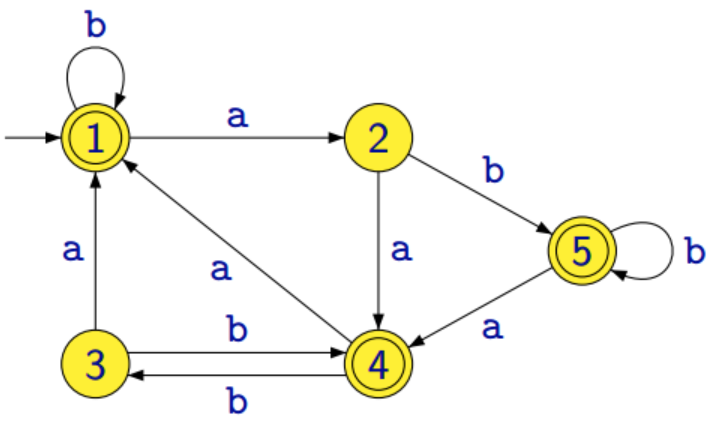
\includegraphics[width=0.5\textwidth]{assets/deter}
	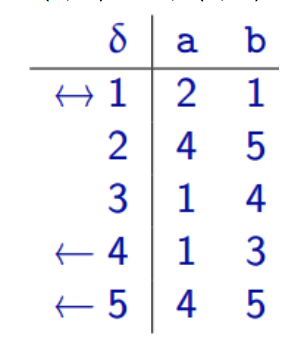
\includegraphics[width=0.2\textwidth]{assets/deter1}
\end{figure}

\subsubsection{Nedeterministický konečný automat (NDKA)}
Formálně je NDKA definován jako pětice $A = (Q, \Sigma, \delta, I, F)$, s tím rozdílem, že oproti deterministickému KA má \textbf{více počátečních stavů} a \textbf{přechodová funkce vrací množinu} stavů:
\begin{itemize}
	\item $\delta$ je přechodová funkce, vrací množinu stavů, $\delta: Q \times \Sigma \rightarrow P(Q)$.
	\item $I$ je konečná množina počátečních stavů, $I \in Q$.
\end{itemize}

\begin{figure}[H]
\centering
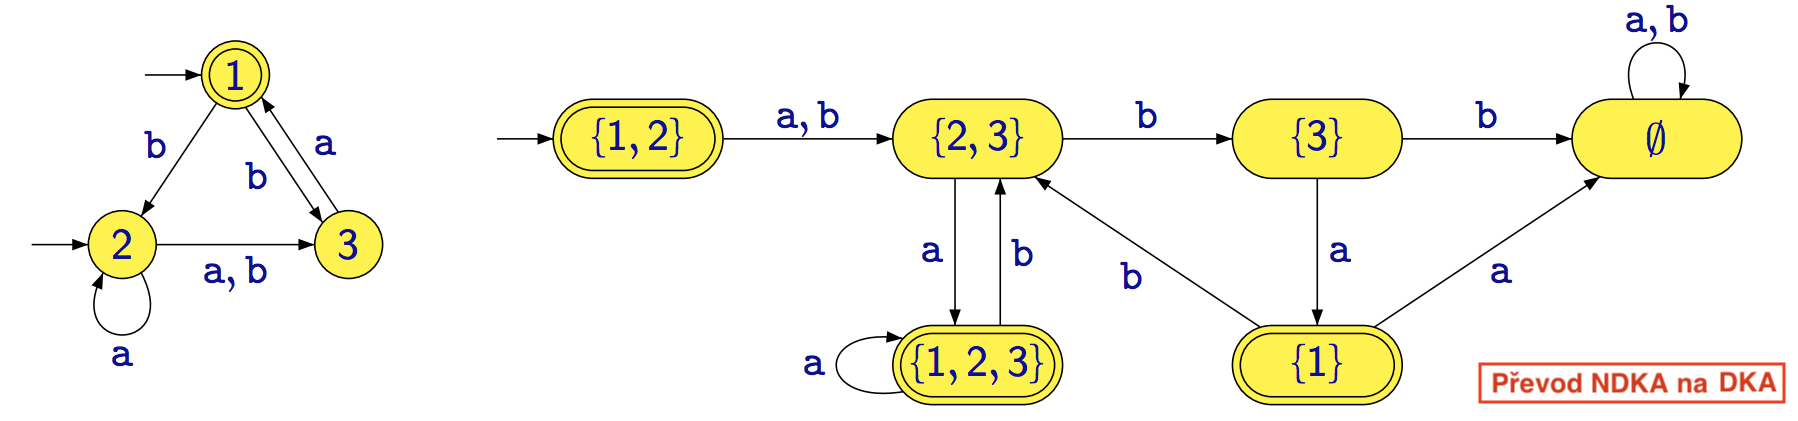
\includegraphics[width=1\textwidth]{assets/nka_na_dka}
\end{figure}

\subsubsection*{Na rozdíl od deterministického automatu:}
\begin{itemize}
	\item Může z jednoho stavu vést \textbf{libovolný počet přechodů} označených stejným symbolem (i \textbf{nulové} $\epsilon$). 
	\item Není zde nutné, aby z každého stavu vystupovaly všechny symboly, které do něj vstoupily $\rightarrow$ \textbf{nemusí ošetřovat všechny varianty}, pouze odhadne, kterou cestou půjde.
	\item Nedeterministický automat přijímá dané slovo, jestliže \textbf{existuje alespoň jeden jeho výpočet}, který vede k přijetí tohoto slova.
	\item V automatu může být \textbf{víc než jeden počáteční stav}.
	\item Lze ho \textbf{převést na deterministický}. Při převodu automatu, který má n stavů může mít výsledný nedeterministický až $2^n$ stavů.
\end{itemize}


\subsubsection{Normovaný tvar}
Začnu v počátečním stavu a procházím navštívené stavy a vytvářím tabulku. Každý KA má \textbf{právě 1} normovaný tvar. Také lze tímto způsobem zjistit, zda jsou automaty \textbf{ekvivalentní}.


\subsection{Regulární výrazy}
Regulární výraz je \textbf{řetězec popisující celou množinu řetězců}, konkrétně \textbf{regulární jazyk}. Regulární výrazy také můžeme chápat jako jednoduchý způsob, jak \textbf{popsat konečný automat} umožňující generovat všechna možná slova patřící do daného jazyka. 

V regulárních výrazech využíváme znaky \textbf{abecedy} a symboly pro \textbf{sjednocení}, \textbf{zřetězení} a \textbf{iterace} regulárních výrazů. Za regulární výraz se považuje i samotný znak abecedy (např. a) stejně jako \textbf{prázdné slovo} $\epsilon$ a \textbf{prázdný jazyk} $\emptyset$.

\subsubsection{Definice regulárních výrazů}
Regulární výrazy popisují jazyky nad abecedou $A = \Sigma: \emptyset, \epsilon, a$ (kde $a \in \Sigma$) jsou regulární výrazy:
\begin{itemize}
	\item $\emptyset$ označuje \textbf{prázdný jazyk},
	\item $\epsilon$ označuje jazyk $\{\epsilon\}$,
	\item $a$ označuje jazyk $\{a\}$.
\end{itemize}
Dále, jestliže $\alpha$, $\beta$ jsou regulární výrazy, pak i $(\alpha + \beta)$, $(\alpha \cdot \beta)$, $(\alpha*)$ jsou regulární výrazy, kde:
\begin{itemize}
	\item $(\alpha + \beta)$ označuje \textbf{sjednocení} jazyků označených $\alpha$ a $\beta$,
	\item $(\alpha \cdot \beta)$ označuje \textbf{zřetězení} jazyků označených $\alpha$ a $\beta$,
	\item $(\alpha*)$ označuje \textbf{iteraci} jazyka označeného $\alpha$.
\end{itemize}
\textbf{Neexistují žádné další regulární výrazy} než ty definované podle předchozích dvou bodů.

\subsubsection*{Příklady}
Ve  všech případech je $\Sigma = \{0, 1\}$:
\begin{itemize}
	\item \textbf{01} (0 a 1) \ldots jazyk tvořený jedním slovem $01$,
	\item \textbf{0+1}  (0 nebo 1) \ldots jazyk tvořený dvěma slovy $0$ a $1$,
	\item \textbf{(01)*}  \ldots jazyk tvořený slovy $\epsilon, 01, 0101, 010101$, \ldots,
	\item \textbf{(0+1)*}  \ldots jazyk tvořený všemi slovy nad abecedou $\{0, 1\}$,
	\item \textbf{(01)*111(01)*}  \ldots jazyk tvořený všemi slovy obsahující podslovo $111$, předcházení i následované libovolným počtem  slov $01$,
	\item \textbf{(0+1)*00+(01)*111(01)*} \ldots jazyk tvořený všemi slovy, která buď končí $00$ nebo obsahují podslovo $111$ předcházené i následované libovolným počtem slov $01$,
	\item \textbf{(0+1)*1(0+1)*} \ldots jazyk tvořený všemi slovy obsahujícími alespoň jeden symbol $1$,
	\item \textbf{0*(10*10*)*} \ldots jazyk tvořený všemi slovy obsahujícími sudý počet symbolů $1$.
\end{itemize}

\subsection{Uzávěrové vlastnosti třídy regulárních jazyků}
\textbf{Uzavřenost množiny nad operací} znamená, že výsledek operace s libovolnými prvky z množiny bude opět spadat do dané množiny. Třídu regulárních jazyků značíme \textbf{REG}. Regulární výrazy (tedy i KA) jsou uzavřené vůči operacím:
\begin{itemize}
	\item \textbf{Sjednocení}, \textbf{průnik}, \textbf{doplněk} -- je-li $L_1, L_2 \in \textrm{REG}$, pak také $L_1 \cup L_2, L_1 \cap L_2, L_1'$ jsou v REG.
	\item \textbf{Zřetězení}, \textbf{iterace} -- je-li $L_1, L_2 \in \textrm{REG}$, pak také $L_1 \cdot L_2, L_1^*$ jsou v REG.
	\item \textbf{Zrcadlový obraz} -- je-li $L \in \textrm{REG}$, pak také $L^R$ jsou v REG.
\end{itemize}

\subsubsection{Operace sjednocení, zřetězení, iterace a zrcadlový obraz u KA}
\begin{itemize}
	\item \textbf{Iterace} -- \textbf{spojíme koncové stavy} jednoho KA s \textbf{počátečními} druhého KA $\epsilon$ přechodem. Na obrázku generuje automat $A^*$ jazyk $L(A^*) = L(A)^*$, který je iterací jazyku generovaného modrého automatu $A$.
	\item \textbf{Zřetězení} -- \textbf{spojíme koncové stavy jednoho} s \textbf{počátečními stavy druhého}. Na obrázku generuje konečný automat $AB$ jazyk $L(AB) = L(A) \cdot L(B)$.
	\begin{figure}[H]
		\centering
		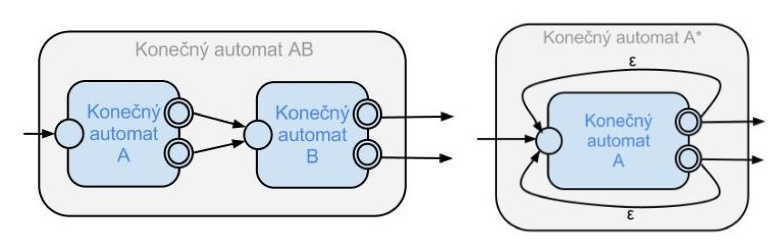
\includegraphics[width=0.7\textwidth]{assets/ka_zret}
	\end{figure}
	\item \textbf{Sjednocení} -- $L(A + B) = L(A) + L(B)$ získáme tak, že vytvoříme \textbf{nový počáteční stav}, ze kterého vedeme $\epsilon$ přechody do počátečních stavů obou automatů. Poté obdobě z koncových stavů obou automatů vedeme $\epsilon$ přechody do \textbf{nového koncového}.
	\item \textbf{Zrcadlový obraz} -- pustíme automat pozpátku, celý jej převrátíme. \textbf{Přehodíme orientaci všech přechodů}, z počátečních stavů uděláme koncové a naopak.
	\begin{figure}[H]
		\centering
		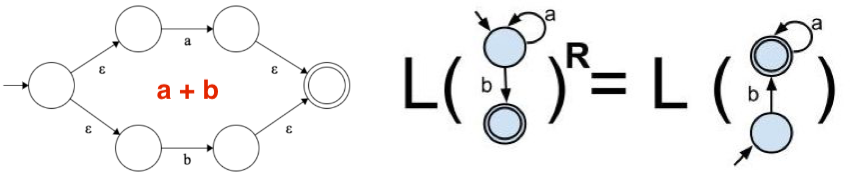
\includegraphics[width=0.8\textwidth]{assets/ka_zrcd}
	\end{figure}
	\item \textbf{Doplněk} -- u DKA provedeme prohození označení příjmajících a ostatních stavů, u NDKA je nejprve nutné provézt převod na DKA.
\end{itemize}
